% -*- latex -*-
%%%%%%%%%%%%%%%%%%%%%%%%%%%%%%%%%%%%%%%%%%%%%%%%%%%%%%%%%%%%%%%%
%%%%%%%%%%%%%%%%%%%%%%%%%%%%%%%%%%%%%%%%%%%%%%%%%%%%%%%%%%%%%%%%
%%%%
%%%% This text file is part of the source of 
%%%% `Introduction to High-Performance Scientific Computing'
%%%% by Victor Eijkhout, copyright 2012-7
%%%%
%%%% This book is distributed under a Creative Commons Attribution 3.0
%%%% Unported (CC BY 3.0) license and made possible by funding from
%%%% The Saylor Foundation \url{http://www.saylor.org}.
%%%%
%%%%
%%%%%%%%%%%%%%%%%%%%%%%%%%%%%%%%%%%%%%%%%%%%%%%%%%%%%%%%%%%%%%%%
%%%%%%%%%%%%%%%%%%%%%%%%%%%%%%%%%%%%%%%%%%%%%%%%%%%%%%%%%%%%%%%%

Gaussian elimination, the use of an $LU$ factorization, is a simple
way to find the solution of a linear system, but as we saw above, in
the sort of problems that come from discretized \ac{PDE}s, it can 
create a lot of fill-in. In this section we will look at a completely
different approach, where the solution of the system is found
by a sequence of approximations.

The computational scheme looks, very roughly, like:
\[
\begin{cases}
  \mbox{Choose any starting vector $x_0$ and repeat for $i\geq0$:}\\
  x_{i+1}=Bx_i+c\\
  \mbox{until some stopping test is satisfied.}
\end{cases}
\]
The important feature here is that no systems are solved with the
original coefficient matrix; instead,
every iteration involves a matrix-vector multiplication or a solution
of a much simpler system. Thus
we have replaced a complicated operation, constructing an $LU$
factorization and solving a system with it, by a repeated simpler
and cheaper operation. This makes iterative methods easier to code,
and potentially more efficient.

Let us consider a simple example to motivate the precise definition of
the iterative methods. Suppose we want to solve the system
\[ \left(\begin{matrix}10&0&1\\ 1/2&7&1\\ 1&0&6\end{matrix}\right)
  \left(
    \begin{matrix}
      x_1\\ x_2\\ x_3
    \end{matrix}\right) = 
    \left(\begin{matrix}
      21\\ 9\\ 8
    \end{matrix}\right)
\]
which has the solution $(2,1,1)$.
%
Suppose you know (for example, from physical considerations) that
solution components are roughly the same size. Observe the
dominant size of the diagonal, then, to decide that
\[ \left(\begin{matrix}10&\\ &7\\ &&6\end{matrix}\right)
  \left(
    \begin{matrix}
      x_1\\ x_2\\ x_3
    \end{matrix}\right) = 
    \left(\begin{matrix}
      21\\ 9\\ 8
    \end{matrix}\right)
\]
might be a good approximation. This has the solution $(2.1,9/7,8/6)$. Clearly,
solving a system that only involves the diagonal of the original
system is both easy to do, and, at least in this case, fairly accurate.

Another approximation to the original system would be to use the lower
triangle. The system
\[ \left(\begin{matrix}10\\ 1/2&7\\ 1&0&6\end{matrix}\right)
  \left(
    \begin{matrix}
      x_1\\ x_2\\ x_3
    \end{matrix}\right) = 
    \left(\begin{matrix}
      21\\ 9\\ 8
    \end{matrix}\right)
\]
has the solution $(2.1,7.95/7,5.9/6)$. Solving triangular systems is a
bit more work than diagonal systems, but still a lot easier than
computing an $LU$ factorization. Also, we have not generated any fill-in
in the process of finding this approximate solution.

Thus we see that there are easy to compute ways of getting
reasonably close to the solution. Can we somehow repeat this trick?

Formulated a bit more abstractly, what we did was instead of solving
$Ax=b$ we solved $L\tilde x=b$. Now define $\Delta x$ as the distance
from the true solution: $\tilde x=x+\Delta x$. This gives $A\Delta
x=A\tilde x-b\equiv r$, where $r$ is the \indexterm{residual}. Next
we solve again $L\widetilde{\Delta x}=r$ and update $\tilde{\tilde
  x}=\tilde x-\widetilde{\Delta x}$.

  \begin{tabular}{|l|ccc|}
    \hline
    iteration&1&2&3\\
    $x_1$&2.1000&2.0017&2.000028\\
    $x_2$&1.1357&1.0023&1.000038\\
    $x_3$&0.9833&0.9997&0.999995\\ \hline
  \end{tabular}

In this case we get two decimals per iteration, which is not typical.

It is now clear why iterative methods can be attractive. 
Solving a system by Gaussian elimination takes $O(n^3)$ operations, as
shown above. A~single iteration in a scheme as the above takes
$O(n^2)$ operations if the matrix is dense, and possibly as low as
$O(n)$ for a sparse matrix. If the number of iterations is low, this makes
iterative methods competitive.

\begin{exercise}
  When comparing iterative and direct methods, the flop count is not
  the only relevant measure. Outline some issues relating to the
  efficiency of the code in both cases. Also compare the cases of
  solving a single linear system and solving multiple.
\end{exercise}

\Level 1 {Abstract presentation}
\label{sec:stationary}

It is time to do a formal presentation of the iterative scheme of the
above example. Suppose we want to solve $Ax=b$, and a direct solution
is too expensive, but multiplying by~$A$ is feasible. Suppose
furthermore that we have a matrix $K\approx A$ such that solving $Kx=b$
can be done cheaply.

Instead of solving $Ax=b$ we solve $Kx=b$, and define $x_0$ as the
solution: $Kx_0=b$. This leaves us with an error $e_0=x_0-x$, for
which we have the equation $A(x_0-e_0)=b$ or $Ae_0=Ax_0-b$. We call
$r_0\equiv Ax_0-b$ the \indexterm{residual}; the error then satisfies
$Ae_0=r_0$.

If we could solve the error from the equation $Ae_0=r_0$, we would be
done: the true solution is then found as $x=x_0-e_0$. However,
since solving with~$A$ was
too expensive the last time, we can not do so this time either, so we
determine the error correction approximately.
We solve $K\tilde e_0=r_0$ and set $x_1:=x_0-\tilde e_0$; the story can now
continue with $e_1=x_1-x$, $r_1=Ax_1-b$, $K\tilde e_1=r_1$,
$x_2=x_1-\tilde e_1$, et cetera.

The iteration scheme is then:
  \begin{quote}
\begin{tabbing}
  Let $x_0$ be given\\
  For $i\geq0$\=:\\
  \>let $r_i=Ax_i-b$\\
  \>compute $e_i$ from $Ke_i=r_i$\\
  \>update $x_{i+1}=x_i-e_i$
\end{tabbing}
  \end{quote}
We call the basic scheme
\begin{equation}
  x_{i+1}=x_i-K\inv r_1
  \label{eq:stat-it}
\end{equation}
a \indexterm{stationary iteration}. It is stationary
because every update is performed the same way, without any dependence
on the iteration number. This scheme has a simple analysis, but
unfortunately limited applicability.

There are several questions we need to answer about iterative schemes:
\begin{itemize}
\item Does this scheme always take us to the solution?
\item If the scheme converges, how quickly?
\item When do we stop iterating?
\item How do we choose $K$?
\end{itemize}
We will now devote some attention to these matters, though a full
discussion is beyond the scope of this book.

\Level 1 {Convergence and error analysis}
\label{sec:stationary-convergence}

We start with the question of whether the iterative scheme converges,
and how quickly. Consider one iteration step:
\begin{equation}
  \begin{array}{r@{{}={}}l}
    r_1&Ax_1-b=A(x_0-\tilde e_0)-b\\
    &r_0-AK\inv r_0\\
    &(I-AK\inv)r_0
  \end{array}
\end{equation}
Inductively we find $r_n=(I-AK\inv)^nr_0$, so $r_n\downarrow0$ if
  all eigenvalues satisfy $|\lambda(I-AK\inv)|<1$\footnote
  {This is fairly easy to see in the case where the matrix is diagonalizable
  and has a full basis of eigenvectors. However, it is true in the general case too.}.

This last statement gives us both a condition for convergence, by
relating $K$ to~$A$, and a geometric convergence rate, if $K$ is
close enough.

\begin{exercise}
  Derive a similar inductive relation for~$e_n$. 
  % Does it give the same convergence criterion?
\end{exercise}

It is hard to determine if the condition $|\lambda(I-AK\inv)|<1$ is
satisfied by computing the actual eigenvalues. However, sometimes the
Gershgorin theorem (appendix~\ref{app:gershgorin}) gives us enough
information.

\begin{exercise}
  Consider the matrix $A$ of equation~\eqref{eq:5starmatrix} that we
  obtained from discretization of a two-dimensional \ac{BVP}. Let $K$
  be matrix containing the diagonal of~$A$, that is $k_{ii}=a_{ii}$
  and $k_{ij}=0$ for~$i\not=j$. Use the Gershgorin theorem to show
  that $|\lambda(I-AK\inv)|<1$.
\end{exercise}

The argument in this exercise is hard to generalize for more
complicated choices of~$K$, such as you will see below.
Here we only remark that for certain matrices $A$, these choices of
$K$ will always lead to convergence, with a speed that decreases as
the matrix size increases. We will not go into the details beyond
stating that for $M$-matrices (see section~\ref{sec:1dbvp}) these
iterative methods converge. For more details on the convergence theory
of stationary iterative methods, see~\cite{Varga:iterative-analysis}

\Level 1 {Computational form}
\label{sec:jacobi-seidel}

Above, in section~\ref{sec:stationary}, we derived stationary
iteration as a process that involves multiplying by~$A$ and solving
with~$K$. However, in some cases a simpler implementation is
possible. Consider the case where $A=K-N$, and we know both $K$
and~$N$. Then we write $Ax=b$ as
\begin{equation}
  Kx=Nx+b
  \label{eq:kx=nx}
\end{equation}
and we observe that an $x$ satisfying~\eqref{eq:kx=nx}
is a fixed point of the iteration
\[ Kx^{(n+1)}=Nx^{(i)}+b. \]
It is easy to see that this is a stationary iteration:
\[
\begin{array}{r@{{}={}}l}
  Kx^{(n+1)}&Nx^{(i)}+b\\ &Kx^{(n)}-Ax^{(n)}+b\\ &Kx^{(n)}-r^{(n)}\\
  \Rightarrow x^{(n+1)} & x^{(n)}-K\inv r^{(n)}.
\end{array}
\]
which is the basic form of equation~\eqref{eq:stat-it}.
%
The convergence criterion $|\lambda(I-AK\inv)|<1$ (see
above) now simplifies to
$|\lambda(NK\inv)|<\nobreak1$.

Let us consider some special cases. First of all, let $K=D_A$, that
is, the matrix containing the diagonal part of~$A$: $k_{ii}=a_{ii}$
and $k_{ij}=0$ for all~\mbox{$i\not=j$}. 
Likewise, $n_{ii}=0$ and $n_{ij}=-a_{ij}$ for all $i\not=\nobreak j$.

This is known as the
\indexterm{Jacobi method} method. The iteration scheme
$Kx^{(n+1)}=Nx^{(n)}+b$
now becomes
\begin{quote}
  \begin{tabbing}
    for \=$t=1,\ldots$ until convergence, do:\\
    \>for \=$i=1\ldots n$:\\
    \>\>{\tt //} $a_{ii}x^{(t+1)}_i = \sum_{j\not=i}
    a_{ij}x^{(t)}_j+b_i$ becomes:\\
    \>\>$x^{(t+1)}_i = a_{ii}\inv(\sum_{j\not=i} a_{ij}x^{(t)}_j+b_i)$
  \end{tabbing}
\end{quote}
(Bearing in mind that divisions are relatively costly,
section~\ref{sec:fp}, we would actually store the $a_{ii}\inv$
quantities explicitly, and replace the division by a multiplication.)

This requires us to have one vector $x$ for the current iterate
$x^{(t)}$, and one temporary~$u$ for the next vector~$x^{(t+1)}$. The
easiest way to write this is probably:
\begin{quote}
  \begin{tabbing}
    for \=$t=1,\ldots$ until convergence, do:\\
    \>for \=$i=1\ldots n$:\\
    \>\>$u_i = a_{ii}\inv (-\sum_{j\not=i} a_{ij}x_j+b_i)$\\
    \>copy $x\leftarrow u$
  \end{tabbing}
\end{quote}
For the simple case of a one-dimensional problem this is illustrated
in figure~\ref{fig:1d-jacobi}:
\begin{figure}[ht]
  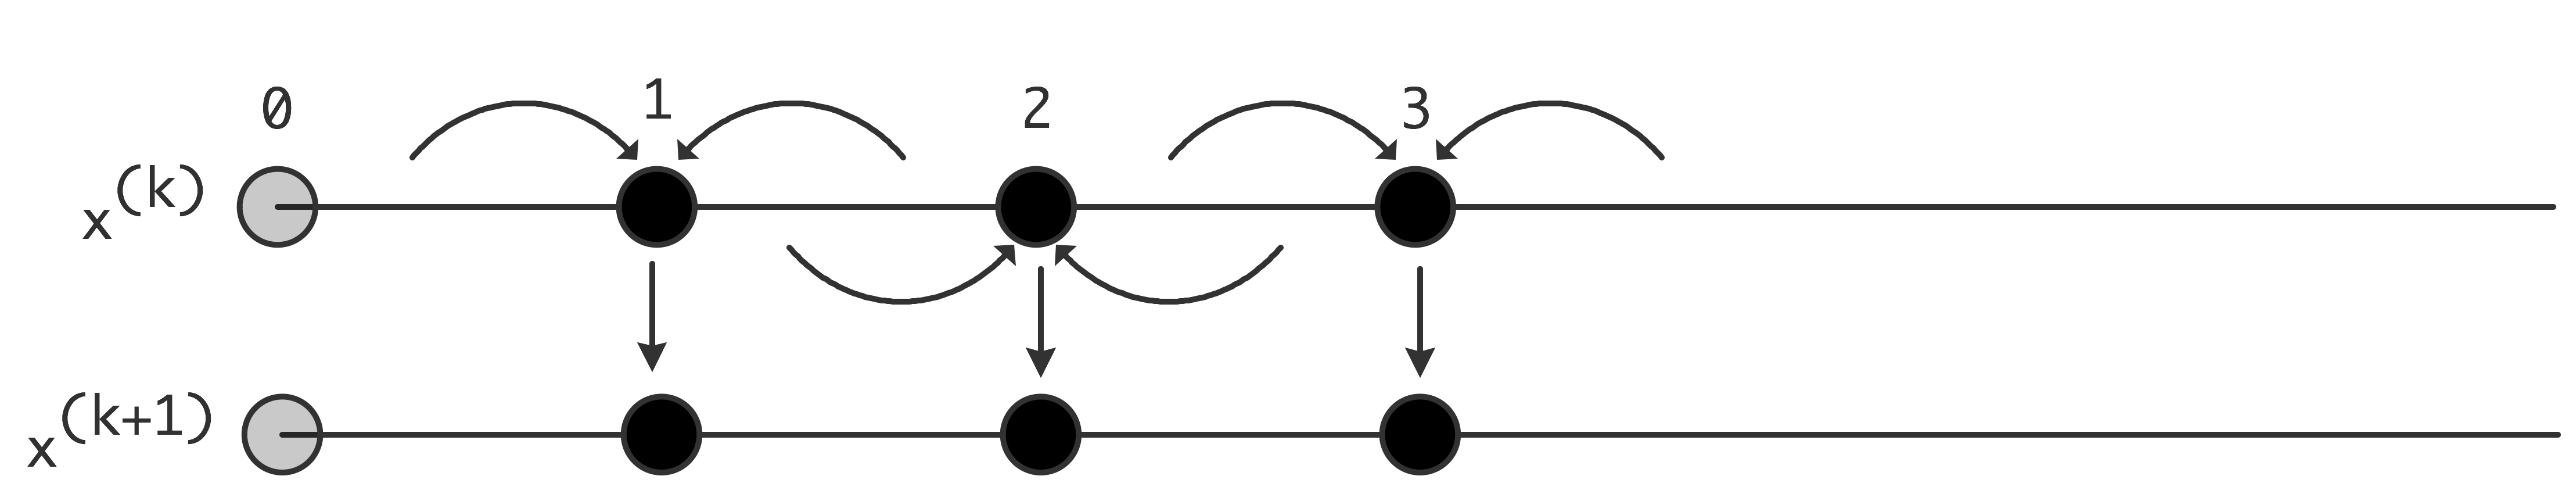
\includegraphics[scale=.08]{graphics/jacobi}
  \caption{Data movement pattern in the Jacobi iteration on a
    one-dimensional problem}
  \label{fig:1d-jacobi}
\end{figure}
in each $x_i$~point the values of the two neighbours are combined with
the current value to generate a new value. Since the computations in
all the $x_i$ points are independent, this can be done
in parallel on a parallel computer.

But, you might think, in the sum $\sum_{j\not=i} a_{ij}x_j$ why
not use the $x^{(t+1)}$ values for as far as already computed?
In terms of the vectors $x^{(t)}$ this means
\begin{quote}
  \begin{tabbing}
    for \=$k=1,\ldots$ until convergence, do:\\
    \>for \=$i=1\ldots n$:\\
    \>\>$x^{(t+1)}_i = a_{ii}\inv (-\sum_{j<i} a_{ij}x_j^{(t+1)} -
                      \sum_{j>i} a_{ij}x_j^{(t)}+b_i)$\\
  \end{tabbing}
\end{quote}
Surprisingly, the implementation is simpler than of the Jacobi method:
\begin{quote}
  \begin{tabbing}
    for \=$t=1,\ldots$ until convergence, do:\\
    \>for \=$i=1\ldots n$:\\
    \>\>$x_i = a_{ii}\inv (-\sum_{j\not=i} a_{ij}x_j +b_i)$\\
  \end{tabbing}
\end{quote}
If you write this out as a matrix equation, you see that
the newly computed elements elements $x^{(t+1)}_i$ are 
multiplied with elements of $D_A+L_A$,
and the old elements $x^{(t)}_j$ by~$U_A$, giving
\[ (D_A+L_A)x^{(k+1)}=-U_Ax^{(k)}+b \]
which is called the \indexterm{Gauss-Seidel} method.

For the one-dimensional case, the Gauss-Seidel method
is illustrated in figure~\ref{fig:1d-sor}; every $x_i$ point
\begin{figure}[ht]
  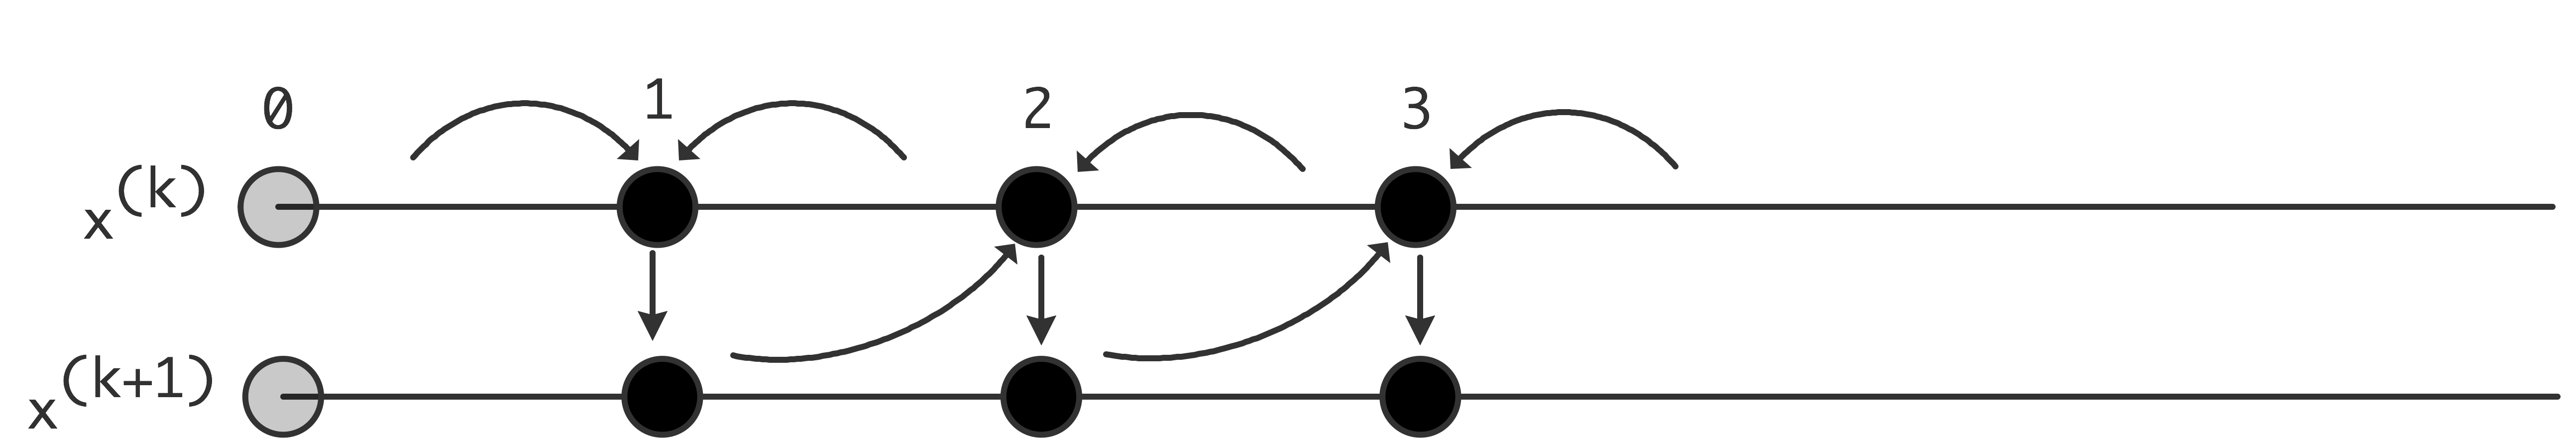
\includegraphics[scale=.08]{graphics/sor}
  \caption{Data movement pattern in the Gauss-Seidel iteration on a
    one-dimensional problem}
  \label{fig:1d-sor}
\end{figure}
still combines its neighbours' values, but now the left value is
actually from the next outer iteration.

Finally, we can insert a damping parameter into the Gauss-Seidel
scheme, giving the \indexacf{SOR} method:
\begin{quote}
  \begin{tabbing}
    for \=$t=1,\ldots$ until convergence, do:\\
    \>for \=$i=1\ldots n$:\\
    \>\>$x^{(t+1)}_i = \omega a_{ii}\inv (-\sum_{j<i} a_{ij}x_j^{(t+1)} -
                      \sum_{j>i} a_{ij}x_j^{(t)} + b_i)
        +(1-\omega)x^{(t)}$\\
  \end{tabbing}
\end{quote}
Surprisingly for something that looks like an interpolation, the
method actually works with value for $\omega$ in the range
$\omega\in(0,2)$, the optimal value being larger
than~$1$~\cite{HaYo:applied}. Computing the optimal $\omega$ is not
simple.

\Level 1 {Convergence of the method}

We are interested in two questions: firstly whether the iterative
method converges at all, and if so, with what speed.  The theory
behind these questions goes far beyond this book. Above we remarked
that convergence can often be guaranteed for $M$-matrices; with regard to
the convergence speed a full analysis is usually only possible in
model cases. For the matrices from \acp{BVP}, as described in
section~\ref{sec:2dbvp}, we state without proof that the smallest
eigenvalue of the coefficient matrix is~$O(h^2)$. The geometric
convergence ratio $|\lambda(I-AK\inv)|$ derived above can then be
shown to be as follows:
\begin{itemize}
\item For the Jacobi method, the ratio is $1-O(h^2)$;
\item For the Gauss-Seidel iteration it also is $1-O(h^2)$, but the
  method converges twice as fast;
\item For the SOR method, the optimal omega can improve the
  convergence factor to~$1-O(h)$.
\end{itemize}

\Level 1 {Jacobi versus Gauss-Seidel and parallelism}

Above, we mostly looked at the Jacobi, Gauss-Seidel, and SOR methods
from a mathematical perspective.
However, such considerations are largely superseded by matters
of parallelization on modern computers.

First we observe that all computations in one iteration of the Jacobi
method are completely independent, so they can simply be vectorized or
done in parallel. That story is different for Gauss-Seidel (and we
ignore SOR from now on, since it only differs from Gauss-Seidel in the
damping  parameter):
since the computation of the
$x_i$ points of one iteration are now dependent, this type of
iteration is not simple
to vectorize or
to implement on a parallel computer.

In many cases, both methods are considered superseded by the \ac{CG}
or \ac{GMRES} methods (sections \ref{sec:cg} and~\ref{sec:gmres}). The
Jacobi method is sometimes used as a preconditioner for these methods.
One place where Gauss-Seidel is still popular is as a
\indextermbus{multigrid}{smoother}. In that case, parallelism is often
found by using a \indexterm{red-black ordering} of the variables.

Further discussion of these issues can be found in section~\ref{sec:parallel-prec}.

\Level 1 {Choice of $K$}
\label{sec:preconditioner}
\index{preconditioner|(}

The convergence and error analysis above showed that the closer $K$ is
to~$A$, the faster the  convergence will be.
%
In the initial examples we already saw the diagonal and lower
triangular choice for~$K$. We can describe these formally by letting
$A=D_A+L_A+U_A$ be a splitting into diagonal, lower triangular, upper
triangular part of~$A$. Here are some methods with their traditional names:
\begin{itemize}
\item Richardson iteration: $K=\alpha I$.
\item Jacobi method: $K=D_A$ (diagonal part),
\item Gauss-Seidel method: $K=D_A+L_A$ (lower triangle, including
  diagonal)
\item The \ac{SOR} method: $K=\omega\inv D_A+ L_A$
\item Symmetric SOR (SSOR) method: $K=(D_A+L_A)D_A\inv(D_A+U_A)$.
\item In \indextermdef{iterative refinement} we let $K=LU$ be
  a true factorization of~$A$. In exact arithmetic, solving a
  system $LUx=y$ gives you the exact solution, so using $K=LU$ in an
  iterative method would give convergence after one step. In practice,
  roundoff error will make the solution be inexact, so people will
  sometimes iterate a few steps to get higher accuracy.
\end{itemize}
\begin{exercise}
  What is the extra cost of a few steps of iterative refinement over a
  single system solution, assuming a dense system?
\end{exercise}

\begin{exercise}
  The Jacobi iteration for the linear system $Ax=b$ is defined as
\[ x_{i+1}=x_i-K^{-1}(Ax_i-b) \]
where $K$ is the diagonal of~$A$. Show that you can transform the
linear system (that is, find a different coefficient matrix and right
hand side vector that will still have the same solution) so that you
can compute the same $x_i$ vectors but with $K=I$, the identity
matrix.

What are the implications of this strategy, in terms of storage and
operation counts? Are there special implications if $A$ is a sparse
matrix?

Suppose $A$ is symmetric. Give a simple example to show that $K^{-1}A$
does not have to be symmetric. Can you come up with a different
transformation of the system so that symmetry of the coefficient
matrix is preserved and that
has the same advantages as the transformation above? You can
assume that the matrix has positive diagonal elements.
\end{exercise}

\begin{exercise}
  Show that the transformation of the previous exercise can also be
  done for the Gauss-Seidel method. Give several reasons why this is
  not a good idea.
\end{exercise}

\begin{remark}
  Stationary iteration can be considered as a form of
  \indextermsub{inexact}{Newton method}, where each iteration uses the
  same approximation to the inverse of the derivative. Standard
  functional analysis results~\cite{Kantorovich:functional} state how
  far this approximation can deviate from the exact inverse.

  A special case is \indexterm{iterative refinement}, where the Newton
  method should converge in one step, but in practice takes multiple
  steps because of roundoff in computer arithmetic. The fact that the
  Newton method will converge as long as the function (or the
  residual) is calculated accurately enough, can be exploited by doing
  the LU solution in lower precision, thus getting higher
  performance~\cite{Dongarra:mixed-refinement}.
\end{remark}

There are  many different ways of choosing the preconditioner
matrix~$K$. Some of them are defined algebraically, such as the
incomplete factorization discussed below. Other choices are inspired
by the differential equation. For instance, if the operator is
\[ \frac\delta{\delta x}(a(x,y)\frac\delta{\delta x}u(x,y)) +
   \frac\delta{\delta y}(b(x,y)\frac\delta{\delta y}u(x,y)) = f(x,y)
\]
then the matrix $K$ could be derived from the operator
\[ \frac\delta{\delta x}(\tilde a(x)\frac\delta{\delta x}u(x,y)) +
   \frac\delta{\delta y}(\tilde b(y)\frac\delta{\delta y}u(x,y)) = f(x,y)
\]
for some choices of $\tilde a,\tilde b$. The second set of equations
is called a \indexterm{separable problem}, and there are
\indexterm{fast solvers} for them, meaning that they have $O(N\log N)$
time complexity; see~\cite{Wi:fastseparable}.

\Level 2 {Constructing $K$ as an incomplete LU factorization}
\label{sec:ilu}

We briefly mention one other choice of~$K$, which is inspired by
Gaussian elimination. As in Gaussian elimination, we let $K=LU$, but
now we use an \indexacf{ILU} factorization. Remember that a
regular $LU$ factorization is expensive because of the fill-in
phenomenon. In an incomplete factorization, we limit the fill-in
artificially.

If we write Gauss elimination as
\begin{verbatim}
for k,i,j:
   a[i,j] = a[i,j] - a[i,k] * a[k,j] / a[k,k]
\end{verbatim}
we define an incomplete variant by
\begin{verbatim}
for k,i,j:
  if a[i,j] not zero:
    a[i,j] = a[i,j] - a[i,k] * a[k,j] / a[k,k]
\end{verbatim}
\begin{itemize}
\item The resulting factorization is no longer exact: $LU\approx A$,
  so it is called an \acf{ILU} factorization.
\item An \ac{ILU} factorization takes much less space than a full
  factorization: the sparsity of $L+U$ is the same as of $A$.
\end{itemize}
The algorithm above is called `ILU(0)', where the zero refers to the
fact that absolutely no fill-in is allowed during the incomplete
factorization.  Other schemes that allow a limited amount of fill-in
exist.  Much more can be said about this method; we will only remark
that for \emph{$M$-matrices}\index{M-matrix}
this scheme typically gives a converging
method~\cite{MevdVo:itsol}.

\begin{exercise}
  How do operation counts of the matrix-vector product and solving a
  system with an \ac{ILU} factorization compare?
\end{exercise}

You have seen that a full factorization of sparse matrix can need a
higher order storage ($N^{3/2}$~for the factorization versus $N$~for
the matrix), but that an incomplete factorization takes~$O(N)$, just
like the matrix. It may therefore come as a surprise that the error
matrix $R=A-LU$ is not dense, but itself sparse.
\begin{exercise}
  Let $A$ be the matrix of the Poisson equation, $LU$~an incomplete
  factorization, and $R=A-LU$. Show that $R$ is a bi-diagonal matrix:
  \begin{itemize}
  \item Consider that $R$ consists of those elements that are
    discarded during the factorization. Where are they located in the
    matrix?
  \item Alternatively, write out the sparsity pattern of the
    product~$LU$ and compare that to the sparsity pattern of~$A$.
  \end{itemize}
\end{exercise}

\Level 2 {Cost of constructing a preconditioner}

In the example of the heat equation (section~\ref{sec:heateq}) you saw
that each time step involves solving a linear system. As an important
practical consequence, any setup cost for solving the linear system,
such as constructing the preconditioner,
will be amortized over the sequence of systems that is to be
solved. A~similar argument holds in the context of nonlinear
equations, a~topic that we will not discuss as such. Nonlinear
equations are solved by an iterative process such as the
\indexterm{Newton method}, which in its multidimensional form leads
to a sequence of linear systems. Although these have different
coefficient matrices, it is again possible to amortize setup costs by
reusing the preconditioner for a number of Newton steps.

\Level 2 {Parallel preconditioners}

Constructing and using a preconditioner is a balancing act of many
considerations: a more accurate preconditioner leads to convergence in
fewer iterations, but these iterations can be more expensive; in
addition, a more accurate preconditioner can be more costly to
construct. In parallel, this story is even more complicated, because
certain preconditioners are not very parallel to begin
with. Therefore, we may accept a preconditioner that is parallel, but
that has a worse iteration count than a serial preconditioner. For
more discussion, see section~\ref{sec:parallel-prec}.

\index{preconditioner|)}

\Level 1 {Stopping tests}

The next question we need to tackle is when to stop iterating. Above
we saw that the error decreases geometrically, so clearly we will
never reach the solution exactly, even if that were possible in
computer arithmetic. Since we only have this relative convergence
behaviour, how do we know when we are close enough?

We would like the error $e_i=x-x_i$ to be small, but measuring this is
impossible. Above we observed that $Ae_i=r_i$, so
\[ \|e_i\|\leq \|A\inv\|\|r_i\| 
    \leq \lambda_{\max}(A\inv)\|r_i\|
\]
If we know anything about the eigenvalues of~$A$, this gives us a
bound on the error. (The norm of~$A$ is only the largest eigenvalue
for symmetric~$A$. In general, we need singular values here.)

Another possibility is to monitor changes in the computed solution. If
these are small:
    \[ \| x_{n+1}-x_n\|/\|x_n\|<\epsilon \]
we can also conclude that we are close to the solution.

\begin{exercise}
  Prove an analytic relationship between the distance between iterates
  and the distance to the true solution. If your equation contains
  constants, can they be determined theoretically or in practice?
\end{exercise}

\begin{exercise}
    Write a simple program to experiment with linear system
    solving. Take the matrix from the 1D BVP (use an efficient storage
    scheme) and program an iterative
    method using the choice $K=D_A$. Experiment with stopping tests on
    the residual and the distance between iterates.
    How does the number of iterations
    depend on the size of the matrix?

    Change the matrix construction so that a certain quantity is
    added the diagonal, that is, add $\alpha I$ to the original
    matrix. What happens when $\alpha>0$? What happens when
    $\alpha<0$? Can you find the value where the behaviour changes?
    Does that value depend on the matrix size?
\end{exercise}
